\section{Latent Dirichlet Allocation}
In PLSA, we will extract a subject word with a fixed probability and then find the corresponding word distribution according to the extracted subject word.Then according to Word distribution, extract a vocabulary.
It can be seen that in PLSA, the topic distribution and word distribution are uniquely determined. However, in LDA, the topic distribution and word distribution are uncertain. The authors of LDA adopt the Bayesian idea that they should obey a distribution. The topic distribution and word distribution are both polynomial distributions, because the polynomial distribution And Dirichlet distribution is a conjugate structure. In LDA, the topic distribution and word distribution use Dirichlet distribution as their conjugate prior distribution.Thus,On the basis of PLSA, LDA adds two Dirichlet priors for topic distribution and word distribution.
\subsection{Generative process of document}
The LDA model can be represented by the following probability graph model:
\begin{figure}[htbp]
% \centering % 图片居中
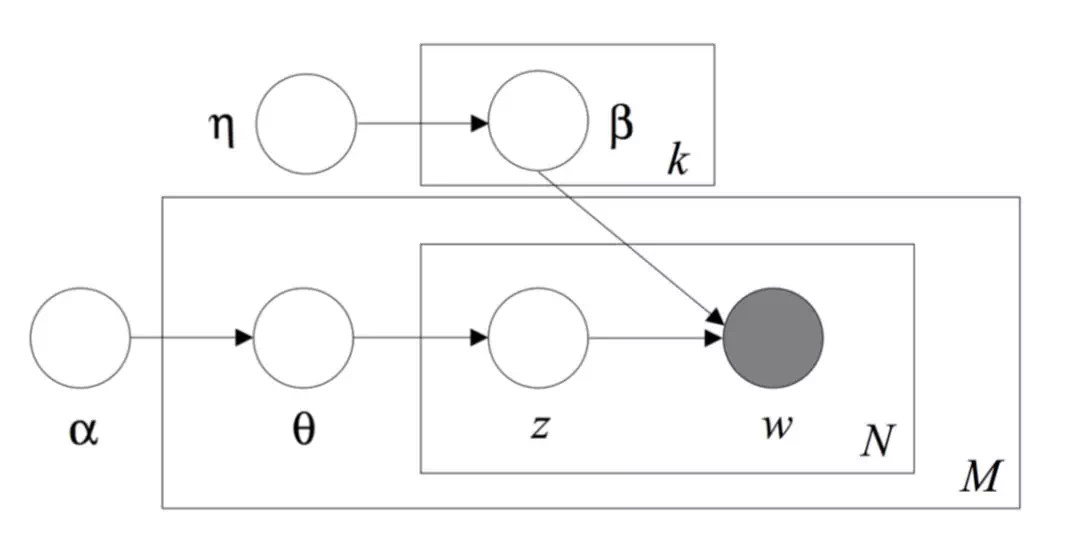
\includegraphics[width = 15cm]{lda.png}
\caption{The caption of this figure.}
\label{fig:figure1label}
\end{figure}


In the LDA model, a document is generated as follows:
\begin{enumerate}
  \item Sampling from Dirichlet distribution $\alpha$ to generate the topic $\theta$ distribution of document $i$.

  \item Sample the $j$th word of the topic $z_{i,j}$  of the document $i$ from the polynomial distribution of topics $\theta_i$.

  \item Sampling from Dirichlet distribution $eta$ to generate word distribution$\beta_{z_{i,j}}$ corresponding to topics$z_{i,j}$.

  \item Sampling from the polynomial distribution$\beta_{z_{i,j}}$  of words to finally generate words $w_{i,j}$.

\end{enumerate}

This probability map can be decomposed into two parts:
\begin{enumerate}
  \item $$\alpha \rightarrow \theta  \rightarrow z $$
This process means that when generating the m-th document, a candidate for a topical toll is generated, and then the topic of each word in the document is randomly generated according to the toll
  \item $$\eta \rightarrow \beta  \rightarrow w|k $$This process means that the word of the document is generated when the topic number is known, and the vector with the topic k is selected in the topic-word matrix, and then the word is generated according to this vector
\end{enumerate}

In the process of document construction,$ M$ documents correspond to $M$ independent Multinomial-Dirichlet conjugate structures, and $K$ topics also correspond to $K$ independent Multinomial-Dirichle conjugate structures. Among them, $M+K$ conjugate structures are all independent. Let’s discuss the document generative process further.


From the first decomposition,We know that $\alpha \rightarrow \theta$ represents the theme corresponding to all documents, which is subject to the Dirichlet distribution. And $\theta  \rightarrow z$  is to generate the theme corresponding to each word, subject to the multinomial distribution. and the Dirichlet distribution is the conjugate distribution of the polynomial distribution. All the whole is a conjugate structure
\begin{eqnarray*}
  f(z_k|\alpha) &=& \int f(z_k|p)f(p|\alpha) d_p \\
              &=& \int \prod_{k=1}^K p_k^{n_k} Dir(p|\alphha) d_p \\
              &=& \int \prod_{k=1}^K p_k^{n_k} \frac{1}{B(\alpha)}\prod_{k=1}^{K}p_k^{\alpha_k-1} d_p \\
              &=& \frac{1}{B(\alpha)}\int \prod_{k=1}{V}p_k^{n_k+\alpha_k-1} d_p \\
              &=& \frac{B(n_k+\alpha_k)}{B(\alpha)}
\end{eqnarray*}
Vector $n = (n_1,_2,..n_K)$ represents the number of words of topic $V$ in each document.
$B$ is the gamma function:
\[
  B(\alpha) = \frac{\prod_{i=1}^V\Gamma(\alpha_i)}{\Gamma(\sum_{i=1}^V \alpha_i)}
\]

For the second decomposition,We know that $\eta \rightarrow \beta$ represents the word-distribution corresponding to all topics, which is subject to the Dirichlet distribution. And $\beta  \rightarrow w|k $  is to generate the word corresponding to each topic, subject to the multinomial distribution. and the Dirichlet distribution is the conjugate distribution of the polynomial distribution. All the whole is a conjugate structure
\begin{eqnarray*}
  f(w|\beta) &=& \int f(w|\beta)f(\beta|\eta) d_{\beta} \\
              &=& \int \prod_{k=1}^V p_k^{n_k} Dir(p|\alpha) d_p \\
              &=& \int \prod_{k=1}^Vp_k^{n_k} \frac{1}{B(\alpha)}\prod_{k=1}^{V}p_k^{\alpha_k-1} d_p \\
              &=& \frac{1}{B(\alpha)}\int \prowd_{k=1}{V}p_k^{n_k+\alpha_k-1} d_p \\
              &=& \frac{B(n_k+\alpha_k)}{B(\alpha)}
\end{eqnarray*}
Vector $n = (n_1,_2,..n_V)$ represents the number of words generated by each topic $V$.

We assume two vector:
\[
  \vec{w} = (\vec{w_1},\vec{w_2},..\vec{w_k})
\]
\[
  \vec{z} = (\vec{z_1},\vec{z_2},..\vec{z_k})
\]


\begin{eqnarray*}
  p(\vec{w}\vec{z}|\alpha,\beta) & = & p(\vec{w}|\vec{z},\beta)p(\vev{z}|\alpha) \\
                                 & = & \prod_i^{K}\frac{B(\beta+n_k)}{\beta}\prod_i^M\frac{n_m+\alpha}{\alpha}
\end{eqnarray*}
$w_k$ indicates that these words were generated by the $k$th topic.

\subsection{Gibbs Sampling for LDA}
BY the joint probability distribution $p(\vec{w}\vec{z}|\alpha,\beta)$ in the previous subsection, we can use Gibbs Sampling to sample it.The $i$th word in the corpus  is denoted as $z_{i}$, where $i=(m,n)$ is a two-dimensional subscript, which corresponds to the $n$th word in the $m$ document. According to the Gibbs Sampling algorithm in the second subsection, we need to require the conditional distribution corresponding to any coordinate axis. Assuming the observed word $w_i=t$, then by Bayes' rule, we can easily get:
\begin{eqnarray*}
  p(z_i=k|\vec{z_{\neg_i}},\vec{w}) & \propto & p(z_i=k,w_i = t|\vec{z_{\neg_i}},\vec{w_{\neg_i}}) \\
  &=& \int p(z_i = k,w_i=t,\theta,\alpha|\vec{z_{\neg_i}},\vec{w_{\neg_i}})d_{\theta} d_{\alpha} \\
  &=& \int p(z_i=k,\theta|\vec{z_{\neg_i}},\vec{w_{\neg_i}}) p(w_i=t,\alpha|\vec{z_{\neg_i}},\vec{w_{\neg_i}})d_{\theta} d_{\alpha}\\
  &=&
\end{eqnarray*}

Finally, we get the Gibbs Sampling formula of the LDA model as:
\[
p(z_i=k|\vec{z_{\neg_i}},\vec{w}) \propto \frac{n_{m,\neg{i}}^{(k)}+\alpha_k}{\sum^K (n_{m,\neg{i})}+\alpha_k)} *
 \frac{n_{k,\neg{i}}^{(t)}+\beta_t}{\sum^V (n_{m,\neg{i})}+\beta_t)}
\]


The equation on the right can be seen as \[
  p(topic|doc)*p(word|topic)
\]


We summarize the LDA Gibbs sampling algorithm process. The first is the training process:
\begin{enumerate}
  \item  Choose the right number of topics 𝐾, choose the right hyperparameter vector 𝛼⃗$\vec{\alpha}$ and $\vec{\beta}$.
 \item Corresponding to each word of each document in the corpus, randomly assign a topic number $z$.
 \item Rescan the corpus, for each word, use Gibbs sampling formula to update its   topic
  \item number, and update the number of the word in the corpus.
Repeat the Gibbs sampling based on coordinate axis rotation in step 3 until the Gibbs sampling converges.
  \item Calculate the theme of each word in each document in the corpus, get the document theme distribution $\theta_d$, calculate the distribution of each theme in the corpus, get the LDA theme and word distribution $\beta_k$.
\end{enumerate}

\subsection{Perplexity and Inference}

In information theory, perplexity is a measure of judging the probability model or probability distribution prediction, and can be used to evaluate the quality of the model.
\[
  perplexity(D) = exp(-\frac{\sum_{k=1}^{M}p(\vec{w_k})}{\sum_{k=1}^{M}N_k})
\]
The denominator is the sum of all the words in the test set, that is, the total length of the test set. Where $p(\vec{w_k})$ refers to the probability of each word of document $k$ in the test set.
\begin{eqnarray*}
  p(\vec{w_k}) &=&\prod_{i=1}^{V}p(w_k^{(i)})\\
               &=&\prod_{i=1}^{V}\int p(w_k^{(i)}|z_i)p(z_i)d_{z_i}
\end{eqnarray*}

With the LDA model, for the new document doc, we only need to think that the topic-word matrix is stable and is provided by the model obtained from the training corpus, so we only need to estimate ttopic distribution of he document. The specific algorithm is as follows:
\begin{enumerate}
  \item  For each word $w_i$ in the current document, randomly initialize a topic number $z$.
  \item Use Gibbs Sampling formula to resample each word $w_i$.
  \item  Repeat the above process until Gibbs Sampling convergence.
  \item Statistics on the topic distribution in the document, the distribution is $\theta_i$.
\end{enumerate}
